\section{Математическое описание}

\subsection{Булева функция.} Булева функция $n$ переменных~--- это отображение $f: \{0, 1\}^n \to \{0, 1\}$. В данной работе рассматривается функция $f(x_1, x_2, x_3, x_4)$ четырёх переменных, заданная вектором значений.

\subsection{Задание функции.} Функция задана десятичным числом 11011, которое в двоичной системе счисления (с дополнением до 16 разрядов) имеет вид:
\[
11011_{10} = 0010101100001011_2.
\]

\subsection{Таблица истинности.} Таблица истинности~--- это способ задания булевой функции, в котором для каждого из $2^n$ наборов значений переменных указано значение функции.

\begin{table}[H]
\centering
\begin{tabular}{|c|c|c|c|c|c|}
\hline
№ & $x_1$ & $x_2$ & $x_3$ & $x_4$ & $f$ \\
\hline
0  & 0 & 0 & 0 & 0 & 0 \\
1  & 0 & 0 & 0 & 1 & 0 \\
2  & 0 & 0 & 1 & 0 & 1 \\
3  & 0 & 0 & 1 & 1 & 0 \\
4  & 0 & 1 & 0 & 0 & 1 \\
5  & 0 & 1 & 0 & 1 & 0 \\
6  & 0 & 1 & 1 & 0 & 1 \\
7  & 0 & 1 & 1 & 1 & 1 \\
8  & 1 & 0 & 0 & 0 & 0 \\
9  & 1 & 0 & 0 & 1 & 0 \\
10 & 1 & 0 & 1 & 0 & 0 \\
11 & 1 & 0 & 1 & 1 & 0 \\
12 & 1 & 1 & 0 & 0 & 1 \\
13 & 1 & 1 & 0 & 1 & 0 \\
14 & 1 & 1 & 1 & 0 & 1 \\
15 & 1 & 1 & 1 & 1 & 1 \\
\hline
\end{tabular}
\caption{Таблица истинности функции $f(x_1, x_2, x_3, x_4)$}
\end{table}

\subsection{Совершенная дизъюнктивная нормальная форма (СДНФ).} СДНФ~--- это представление булевой функции в виде дизъюнкции минтермов. Минтерм~--- это конъюнкция, в которой каждая переменная функции встречается ровно один раз (с отрицанием или без). Для набора $(a_1, a_2, a_3, a_4)$, на котором функция равна 1, минтерм имеет вид:
\[
m_i = x_1^{a_1} \land x_2^{a_2} \land x_3^{a_3} \land x_4^{a_4},
\]
где $x_j^{1} = x_j$, $x_j^{0} = \overline{x_j}$.

СДНФ заданной функции:
\begin{multline*}
f = \overline{x_1}\,\overline{x_2}\,x_3\,\overline{x_4} \lor \overline{x_1}\,x_2\,\overline{x_3}\,\overline{x_4} \lor \overline{x_1}\,x_2\,x_3\,\overline{x_4} \lor \overline{x_1}\,x_2\,x_3\,x_4 \lor {} \\
{} \lor x_1\,x_2\,\overline{x_3}\,\overline{x_4} \lor x_1\,x_2\,x_3\,\overline{x_4} \lor x_1\,x_2\,x_3\,x_4
\end{multline*}

\subsection{Дизъюнктивная нормальная форма (ДНФ).} ДНФ~--- это представление булевой функции в виде дизъюнкции конъюнкций. В отличие от СДНФ, конъюнкции в ДНФ могут содержать не все переменные функции.

\subsection{Минимальная ДНФ.} Минимальная ДНФ~--- это ДНФ с наименьшим числом литералов. Для её нахождения используется минимизация СДНФ.

Минимальная ДНФ заданной функции:
\[
f = \overline{x_1}\,x_3\,\overline{x_4} \lor x_2\,\overline{x_4} \lor x_2\,x_3
\]

\subsection{Выбор порядка переменных.} Порядок следования переменных выбирается с целью получения наиболее компактной бинарной диаграммы решений. 

Проанализируем влияние каждой переменной на функцию. Из таблицы истинности видно, что:
\begin{itemize}
    \item при $x_2 = 0$ и $x_1 = 1$ функция всегда равна 0 (наборы 8--11);
    \item при $x_2 = 1$ поведение функции одинаково для $x_1 = 0$ и $x_1 = 1$ (наборы 4--7 и 12--15 дают одинаковые значения: 1, 0, 1, 1);
    \item переменная $x_4$ определяет значение функции при фиксированных остальных: $f = 1$ только при $x_4 = 0$ (за исключением наборов 7 и 15, где $x_2 = x_3 = 1$).
\end{itemize}

Выберем порядок $x_2, x_1, x_3, x_4$.
\begin{itemize}
    \item $x_2$ на первом месте: при $x_2 = 1$ левая и правая части дерева (по $x_1$) идентичны, что позволяет объединить подграфы;
    \item $x_1$ на втором месте: при $x_2 = 0$ переменная $x_1$ разделяет функцию на тривиальную часть ($x_1 = 1 \Rightarrow f = 0$) и нетривиальную;
    \item $x_4$ в конце: часто определяет финальное значение ($f = 1$ преимущественно при $x_4 = 0$), что даёт возможность объединить листья.
\end{itemize}

\subsection{Семантическое дерево.} Таблицу истинности булевой функции $n$ переменных можно представить в виде бинарного дерева высоты $n+1$. Ярусы дерева соответствуют переменным, дуги~--- значениям переменных (пунктирная линия~--- 0, сплошная~--- 1), а листья хранят значения функции на кортеже, соответствующем пути из корня в этот лист.

Семантическое дерево для заданной функции представлено на рис.~\ref{fig:semantic-tree}, упрощённое семантическое дерево~--- на рис.~\ref{fig:bdd}.

\begin{figure}[H]
\centering
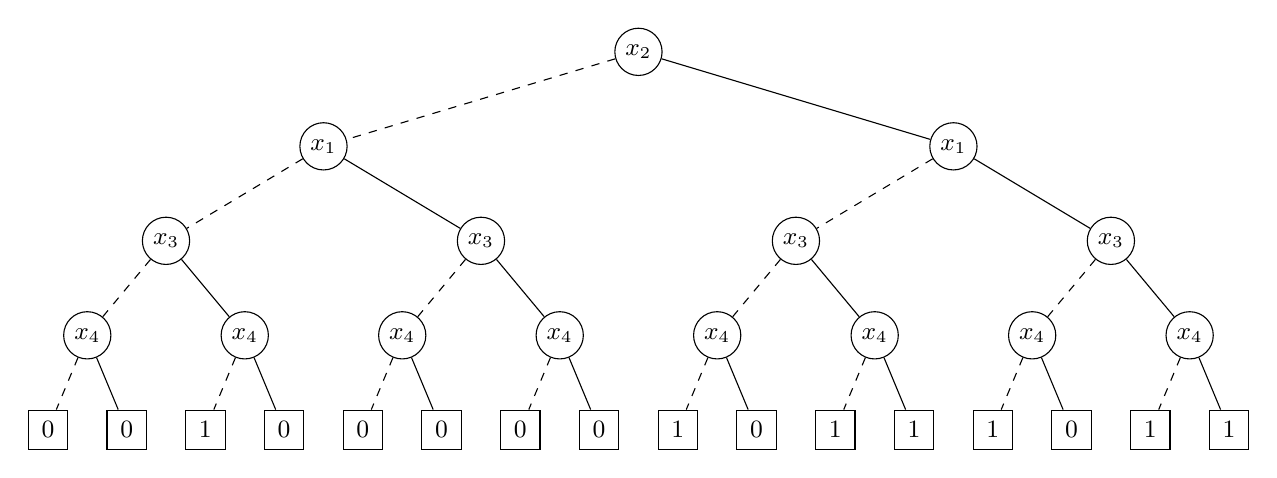
\begin{tikzpicture}[
    level 1/.style={sibling distance=80mm, level distance=12mm},
    level 2/.style={sibling distance=40mm, level distance=12mm},
    level 3/.style={sibling distance=20mm, level distance=12mm},
    level 4/.style={sibling distance=10mm, level distance=12mm},
    every node/.style={circle, draw, solid, minimum size=6mm, inner sep=1pt, font=\small},
    leaf/.style={rectangle, draw, solid, minimum size=5mm, inner sep=2pt, font=\small},
    edge0/.style={dashed},
    edge1/.style={solid}
]
\node {$x_2$}
    child {node {$x_1$}
        child {node {$x_3$}
            child {node {$x_4$}
                child {node[leaf] {0} edge from parent[edge0]}
                child {node[leaf] {0} edge from parent[edge1]}
                edge from parent[edge0]
            }
            child {node {$x_4$}
                child {node[leaf] {1} edge from parent[edge0]}
                child {node[leaf] {0} edge from parent[edge1]}
                edge from parent[edge1]
            }
            edge from parent[edge0]
        }
        child {node {$x_3$}
            child {node {$x_4$}
                child {node[leaf] {0} edge from parent[edge0]}
                child {node[leaf] {0} edge from parent[edge1]}
                edge from parent[edge0]
            }
            child {node {$x_4$}
                child {node[leaf] {0} edge from parent[edge0]}
                child {node[leaf] {0} edge from parent[edge1]}
                edge from parent[edge1]
            }
            edge from parent[edge1]
        }
        edge from parent[edge0]
    }
    child {node {$x_1$}
        child {node {$x_3$}
            child {node {$x_4$}
                child {node[leaf] {1} edge from parent[edge0]}
                child {node[leaf] {0} edge from parent[edge1]}
                edge from parent[edge0]
            }
            child {node {$x_4$}
                child {node[leaf] {1} edge from parent[edge0]}
                child {node[leaf] {1} edge from parent[edge1]}
                edge from parent[edge1]
            }
            edge from parent[edge0]
        }
        child {node {$x_3$}
            child {node {$x_4$}
                child {node[leaf] {1} edge from parent[edge0]}
                child {node[leaf] {0} edge from parent[edge1]}
                edge from parent[edge0]
            }
            child {node {$x_4$}
                child {node[leaf] {1} edge from parent[edge0]}
                child {node[leaf] {1} edge from parent[edge1]}
                edge from parent[edge1]
            }
            edge from parent[edge1]
        }
        edge from parent[edge1]
    };
\end{tikzpicture}
\caption{Семантическое дерево функции $f$}
\label{fig:semantic-tree}
\end{figure}

\begin{figure}[H]
\centering
\begin{tikzpicture}[
    level 1/.style={sibling distance=50mm, level distance=15mm},
    level 2/.style={sibling distance=25mm, level distance=15mm},
    level 3/.style={sibling distance=15mm, level distance=15mm},
    node/.style={circle, draw, solid, minimum size=8mm, inner sep=1pt, font=\small},
    leaf/.style={rectangle, draw, solid, minimum size=7mm, inner sep=2pt, font=\small},
    edge0/.style={dashed},
    edge1/.style={solid}
]
\node[node] {$x_2$}
    child {node[node] {$x_1$}
        child {node[node] {$x_3$}
            child {node[leaf] {0} edge from parent[edge0]}
            child {node[node] {$x_4$} 
                child {node[leaf] {1} edge from parent[edge0]}
                child {node[leaf] {0} edge from parent[edge1]}
                edge from parent[edge1]
            }
            edge from parent[edge0]
        }
        child {node[leaf] {0} edge from parent[edge1]}
        edge from parent[edge0]
    }
    child {node[node] {$x_3$}
        child {node[node] {$x_4$}
            child {node[leaf] {1} edge from parent[edge0]}
            child {node[leaf] {0} edge from parent[edge1]}
            edge from parent[edge0]
        }
        child {node[leaf] {1} edge from parent[edge1]}
        edge from parent[edge1]
    };
\end{tikzpicture}
\caption{Упрощённое семантическое дерево функции $f$}
\label{fig:bdd}
\end{figure}

Бинарная диаграмма решений для заданной функции представлена на рис.~\ref{fig:bdd-graph} (пунктирная линия~--- 0, сплошная линия~--- 1).

\begin{figure}[H]
\centering
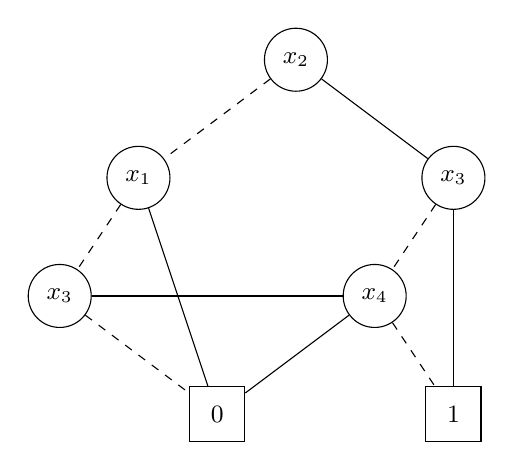
\begin{tikzpicture}[
    node/.style={circle, draw, solid, minimum size=8mm, inner sep=1pt, font=\small},
    leaf/.style={rectangle, draw, solid, minimum size=7mm, inner sep=2pt, font=\small},
    edge0/.style={dashed},
    edge1/.style={solid}
]
% Уровень 1
\node[node] (x2) at (0, 0) {$x_2$};

% Уровень 2
\node[node] (x1) at (-2, -1.5) {$x_1$};
\node[node] (x3b) at (2, -1.5) {$x_3$};

% Уровень 3
\node[node] (x3a) at (-3, -3) {$x_3$};
\node[node] (x4a) at (1, -3) {$x_4$};

% Листья
\node[leaf] (l0) at (-1, -4.5) {0};
\node[leaf] (l1) at (2, -4.5) {1};

% Рёбра от x2
\draw[edge0] (x2) -- (x1);
\draw[edge1] (x2) -- (x3b);

% Рёбра от x1
\draw[edge0] (x1) -- (x3a);
\draw[edge1] (x1) -- (l0);

% Рёбра от x3a
\draw[edge0] (x3a) -- (l0);
\draw[edge1] (x3a) -- (x4a);

% Рёбра от x3b
\draw[edge0] (x3b) -- (x4a);
\draw[edge1] (x3b) -- (l1);

% Рёбра от x4a
\draw[edge0] (x4a) -- (l1);
\draw[edge1] (x4a) -- (l0);
\end{tikzpicture}
\caption{Бинарная диаграмма решений}
\label{fig:bdd-graph}
\end{figure}

\subsection{Синтаксическое дерево минимальной ДНФ.} Синтаксическое дерево~--- это представление формулы в виде дерева, где внутренние вершины соответствуют операциям, а листья~--- переменным или константам.

Синтаксическое дерево для минимальной ДНФ $f = \overline{x_1}\,x_3\,\overline{x_4} \lor x_2\,\overline{x_4} \lor x_2\,x_3$ представлено на рис.~\ref{fig:syntax-tree}.

\begin{figure}[H]
\centering
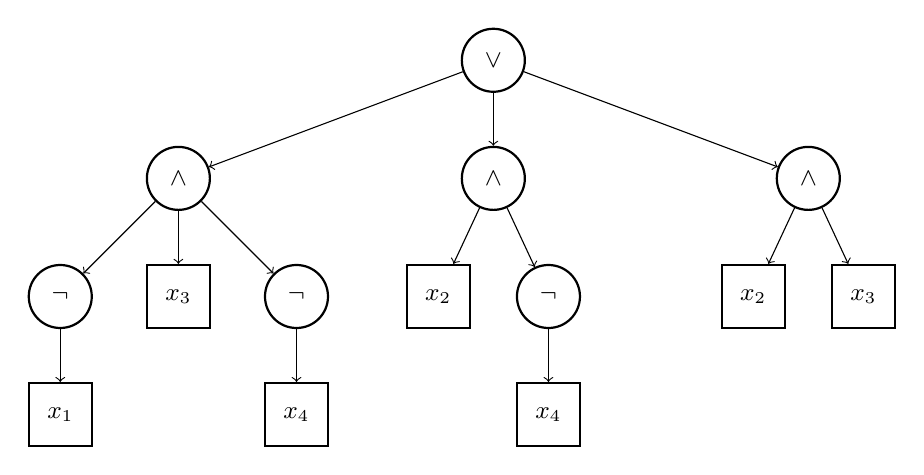
\begin{tikzpicture}[
    op/.style={circle, draw, thick, minimum size=8mm, font=\small},
    var/.style={rectangle, draw, thick, minimum size=8mm, font=\small},
    edge0/.style={dashed},
    edge1/.style={solid},
]

% Уровень 0: корень
\node[op] (root) at (0, 0) {$\lor$};

% Уровень 1: три конъюнкции
\node[op] (and1) at (-4, -1.5) {$\land$};
\node[op] (and2) at (0, -1.5) {$\land$};
\node[op] (and3) at (4, -1.5) {$\land$};

% Уровень 2: операнды первой конъюнкции
\node[op] (neg1) at (-5.5, -3) {$\neg$};
\node[var] (x3a) at (-4, -3) {$x_3$};
\node[op] (neg2) at (-2.5, -3) {$\neg$};

% Уровень 2: операнды второй конъюнкции
\node[var] (x2a) at (-0.7, -3) {$x_2$};
\node[op] (neg3) at (0.7, -3) {$\neg$};

% Уровень 2: операнды третьей конъюнкции
\node[var] (x2b) at (3.3, -3) {$x_2$};
\node[var] (x3b) at (4.7, -3) {$x_3$};

% Уровень 3: переменные под отрицаниями
\node[var] (x1) at (-5.5, -4.5) {$x_1$};
\node[var] (x4a) at (-2.5, -4.5) {$x_4$};
\node[var] (x4b) at (0.7, -4.5) {$x_4$};

% Рёбра от корня
\draw[->] (root) -- (and1);
\draw[->] (root) -- (and2);
\draw[->] (root) -- (and3);

% Рёбра первой конъюнкции
\draw[->] (and1) -- (neg1);
\draw[->] (and1) -- (x3a);
\draw[->] (and1) -- (neg2);

% Рёбра второй конъюнкции
\draw[->] (and2) -- (x2a);
\draw[->] (and2) -- (neg3);

% Рёбра третьей конъюнкции
\draw[->] (and3) -- (x2b);
\draw[->] (and3) -- (x3b);

% Рёбра отрицаний
\draw[->] (neg1) -- (x1);
\draw[->] (neg2) -- (x4a);
\draw[->] (neg3) -- (x4b);

\end{tikzpicture}
\caption{Синтаксическое дерево минимальной ДНФ}
\label{fig:syntax-tree}
\end{figure}

\subsection{Производная булевой функции.} Производная булевой функции $f$ по переменной $x_i$:
\[
\frac{\partial f}{\partial x_i} = f|_{x_i = 0} \oplus f|_{x_i = 1}.
\]

Вычислим производные функции $f = \overline{x_1}\,x_3\,\overline{x_4} \lor x_2\,\overline{x_4} \lor x_2\,x_3$ по каждой переменной.

\textbf{Производная по $x_1$:}
\begin{align*}
f|_{x_1=0} &= x_3\,\overline{x_4} \lor x_2\,\overline{x_4} \lor x_2\,x_3 \\
f|_{x_1=1} &= x_2\,\overline{x_4} \lor x_2\,x_3 \\
\frac{\partial f}{\partial x_1} &= \overline{x_2}\,x_3\,\overline{x_4}
\end{align*}

\textbf{Производная по $x_2$:}
\begin{align*}
f|_{x_2=0} &= \overline{x_1}\,x_3\,\overline{x_4} \\
f|_{x_2=1} &= \overline{x_1}\,x_3\,\overline{x_4} \lor \overline{x_4} \lor x_3 = \overline{x_4} \lor x_3 \\
\frac{\partial f}{\partial x_2} &= x_1\,\overline{x_4} \lor x_1\,x_3 \lor \overline{x_3}\,\overline{x_4} \lor x_3\,x_4
\end{align*}

\textbf{Производная по $x_3$:}
\begin{align*}
f|_{x_3=0} &= x_2\,\overline{x_4} \\
f|_{x_3=1} &= \overline{x_1}\,\overline{x_4} \lor x_2\,\overline{x_4} \lor x_2 = \overline{x_1}\,\overline{x_4} \lor x_2 \\
\frac{\partial f}{\partial x_3} &= \overline{x_1}\,\overline{x_4} \lor x_2\,x_4
\end{align*}

\textbf{Производная по $x_4$:}
\begin{align*}
f|_{x_4=0} &= \overline{x_1}\,x_3 \lor x_2 \lor x_2\,x_3 = \overline{x_1}\,x_3 \lor x_2 \\
f|_{x_4=1} &= x_2\,x_3 \\
\frac{\partial f}{\partial x_4} &= \overline{x_1}\,x_3 \lor x_2\,\overline{x_3}
\end{align*}